\documentclass[11pt]{article}
\usepackage{amsmath}
\usepackage{amssymb}
\usepackage{graphicx}
\usepackage{tabularx}
\usepackage{fancyhdr}
\usepackage{lastpage}

% Page layout
\usepackage[top=1in, bottom=1in, left=1in, right=1in]{geometry}

% Header and footer
\pagestyle{fancy}
\fancyhf{}
\rfoot{Page \thepage}
\renewcommand{\headrulewidth}{0pt}

% Modified Question command with left-aligned number
\newcommand{\questiona}[2]{
    \noindent\textbf{Q#2.} #1 \hfill \textbf{[1 Mark]}
}

\newcommand{\questionb}[2]{
    \noindent\textbf{Q#2.} #1 \hfill \textbf{[2 Marks]}
}

\begin{document}

% Title section with horizontal line
\begin{center}
    \Large\textbf{GATE 2017 - Mathematics (MA)} \\
    \large\textbf{General Aptitude and Technical Questions} \\
    \rule{\textwidth}{0.5pt} % Horizontal line below heading
\end{center}

\vspace{0.5cm}

% General Aptitude Section
\section*{General Aptitude}

\questiona{The ninth and the tenth of this month are Monday and Tuesday \_\_\_\_\_.}{1}
\begin{enumerate}
    \item[(A)] figuratively  
    \item[(B)] retrospectively  
    \item[(C)] respectively  
    \item[(D)] rightfully  
\end{enumerate}
\vspace{0.5cm}

\questiona{It is \_\_\_\_\_ to read this year's textbook \_\_\_\_\_ the last year's.}{2}
\begin{enumerate}
    \item[(A)] easier, than  
    \item[(B)] most easy, than  
    \item[(C)] easier, from  
    \item[(D)] easiest, from  
\end{enumerate}
\vspace{0.5cm}

\questiona{A rule states that in order to drink beer, one must be over 18 years old. In a bar, there are 4 people. P is 16 years old, Q is 25 years old, R is drinking milkshake and S is drinking a beer. What must be checked to ensure that the rule is being followed?}{3}
\begin{enumerate}
    \item[(A)] Only P's drink  
    \item[(B)] Only P's drink and S's age  
    \item[(C)] Only S's age  
    \item[(D)] Only P's drink, Q's drink and S's age  
\end{enumerate}
\vspace{0.5cm}

\questiona{Fatima starts from point P, goes North for 3 km, and then East for 4 km to reach point Q. She then turns to face point P and goes 15 km in that direction. She then goes North for 6 km. How far is she from point P, and in which direction should she go to reach point P?}{4}
\begin{enumerate}
    \item[(A)] 8 km, East  
    \item[(B)] 12 km, North  
    \item[(C)] 6 km, East  
    \item[(D)] 10 km, North  
\end{enumerate}
\vspace{0.5cm}

\questiona{500 students are taking one or more courses out of Chemistry, Physics, and Mathematics. Registration records indicate course enrolment as follows: Chemistry (329), Physics (186), Mathematics (295), Chemistry and Physics (83), Chemistry and Mathematics (217), and Physics and Mathematics (63). How many students are taking all 3 subjects?}{5}
\begin{enumerate}
    \item[(A)] 37  
    \item[(B)] 43  
    \item[(C)] 47  
    \item[(D)] 53  
\end{enumerate}
\vspace{0.5cm}

\questionb{"If you are looking for a history of India, or for an account of the rise and fall of the British Raj, or for the reason of the cleaving of the subcontinent into two mutually antagonistic parts and the effects this mutilation will have in the respective sections, and ultimately on Asia, you will not find it in these pages; for though I have spent a lifetime in the country, I lived too near the seat of events, and was too intimately associated with the actors, to get the perspective needed for the impartial recording of these matters." Which of the following statements best reflects the author's opinion?}{6}
\begin{enumerate}
    \item[(A)] An intimate association does not allow for the necessary perspective.  
    \item[(B)] Matters are recorded with an impartial perspective.  
    \item[(C)] An intimate association offers an impartial perspective.  
    \item[(D)] Actors are typically associated with the impartial recording of matters.  
\end{enumerate}
\vspace{0.5cm}

\questionb{Each of P, Q, R, S, W, X, Y and Z has been married at most once. X and Y are married and have two children P and Q. Z is the grandfather of the daughter S of P. Further, Z and W are married and are parents of R. Which one of the following must necessarily be FALSE?}{7}
\begin{enumerate}
    \item[(A)] X is the mother-in-law of R  
    \item[(B)] P and R are not married to each other  
    \item[(C)] P is a son of X and Y  
    \item[(D)] Q cannot be married to R  
\end{enumerate}
\vspace{0.5cm}

\questionb{1200 men and 500 women can build a bridge in 2 weeks. 900 men and 250 women will take 3 weeks to build the same bridge. How many men will be needed to build the bridge in one week?}{8}
\begin{enumerate}
    \item[(A)] 3000  
    \item[(B)] 3300  
    \item[(C)] 3600  
    \item[(D)] 3900  
\end{enumerate}
\vspace{0.5cm}

\questionb{The number of 3-digit numbers such that the digit 1 is never to the immediate right of 2 is}{9}
\begin{enumerate}
    \item[(A)] 781  
    \item[(B)] 791  
    \item[(C)] 881  
    \item[(D)] 891  
\end{enumerate}
\vspace{0.5cm}

\questionb{A contour line joins locations having the same height above the mean sea level. The following is a contour plot of a geographical region. Contour lines are shown at 25 m intervals in this plot. Which of the following is the steepest path leaving from P?}{10}
\begin{center}
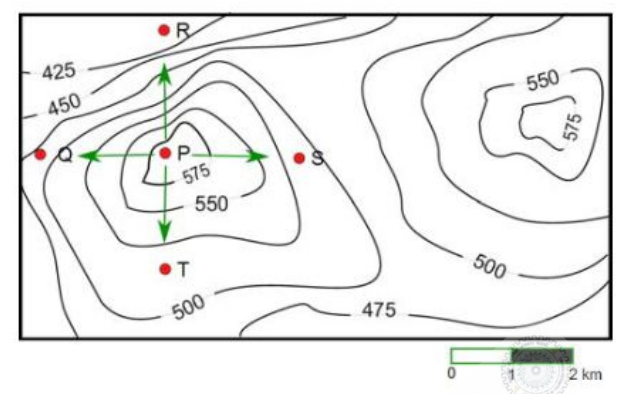
\includegraphics[width=0.5\textwidth]{figures/10.png}
\end{center}
\begin{enumerate}
    \item[(A)] P to Q  
    \item[(B)] P to R  
    \item[(C)] P to S  
    \item[(D)] P to T  
\end{enumerate}
\vspace{0.5cm}

% Technical Section
\section*{Technical Section (Mathematics)}

\questiona{Consider the vector space \( V = \{a_0 + a_1 x + a_2 x^2 : a_i \in \mathbb{R} \text{ for } i = 0, 1, 2\} \) of polynomials of degree at most 2. Let \( f: V \to \mathbb{R} \) be a linear functional such that \( f(1+x) = 0 \), \( f(1-x^2) = 0 \) and \( f(x^2 - x) = 2 \). Then \( f(1+x+x^2) \) equals \_\_\_\_\_.}{1}
\vspace{0.5cm}

\questiona{Let \( A \) be a \( 7 \times 7 \) matrix such that \( 2A^2 - A^4 = I \), where \( I \) is the identity matrix. If \( A \) has two distinct eigenvalues and each eigenvalue has geometric multiplicity 3, then the total number of nonzero entries in the Jordan canonical form of \( A \) equals \_\_\_\_\_.}{2}
\vspace{0.5cm}

\questiona{Let \( f(z) = (x^2 + y^2) + i 2xy \) and \( g(z) = 2xy + i(y^2 - x^2) \) for \( z = x + iy \in \mathbb{C} \). Then, in the complex plane \( \mathbb{C} \),}{3}
\begin{enumerate}
    \item[(A)] \( f \) is analytic and \( g \) is NOT analytic  
    \item[(B)] \( f \) is NOT analytic and \( g \) is analytic  
    \item[(C)] neither \( f \) nor \( g \) is analytic  
    \item[(D)] both \( f \) and \( g \) are analytic  
\end{enumerate}
\vspace{0.5cm}

\questiona{If \[ \sum_{n=-\infty}^{\infty} a_n (z-2)^n \] is the Laurent series of the function \[ f(z) = \frac{z^4 + z^3 + z^2}{(z-2)^3} \] for \( z \in \mathbb{C} \setminus \{2\} \), then \( a_{-2} \) equals \_\_\_\_\_.}{4}
\vspace{0.5cm}

\questiona{Let \( f_n: [0,1] \to \mathbb{R} \) be given by \( f_n(x) = \frac{2x^2}{x^2 + (1 - 2nx)^2}, n = 1, 2, \ldots \). Then the sequence \( (f_n) \)}{5}
\begin{enumerate}
    \item[(A)] converges uniformly on \([0,1]\)  
    \item[(B)] does NOT converge uniformly on \([0,1]\) but has a subsequence that converges uniformly on \([0,1]\)  
    \item[(C)] does NOT converge pointwise on \([0,1]\)  
    \item[(D)] converges pointwise on \([0,1]\) but does NOT have a subsequence that converges uniformly on \([0,1]\)  
\end{enumerate}
\vspace{0.5cm}

\questiona{Let \( C: x^2 + y^2 = 9 \) be the circle in \(\mathbb{R}^2\) oriented positively. Then \[\frac{1}{\pi} \oint_C \left( 3y - e^{\cos x^2} \right) dx + \left( 7x + \sqrt{y^4 + 11} \right) dy\] equals \_\_\_\_\_.}{6}
\vspace{0.5cm}

\questiona{Consider the following statements:  
(P): There exists an unbounded subset of \(\mathbb{R}\) whose Lebesgue measure is equal to 5.  
(Q): If \( f : \mathbb{R} \to \mathbb{R} \) is continuous and \( g : \mathbb{R} \to \mathbb{R} \) is such that \( f = g \) almost everywhere on \(\mathbb{R}\), then \( g \) must be continuous almost everywhere on \(\mathbb{R}\).  
Which of the above statements hold TRUE?}{7}
\begin{enumerate}
    \item[(A)] Both P and Q  
    \item[(B)] Only P  
    \item[(C)] Only Q  
    \item[(D)] Neither P nor Q  
\end{enumerate}
\vspace{0.5cm}

\questiona{If \( x^3 y^2 \) is an integrating factor of \( \left( 6y^2 + axy \right) dx + \left( 6xy + bx^2 \right) dy = 0 \), where \( a, b \in \mathbb{R} \), then}{8}
\begin{enumerate}
    \item[(A)] \( 3a - 5b = 0 \)  
    \item[(B)] \( 2a - b = 0 \)  
    \item[(C)] \( 3a + 5b = 0 \)  
    \item[(D)] \( 2a + b = 0 \)  
\end{enumerate}
\vspace{0.5cm}

\questiona{If \( x(t) \) and \( y(t) \) are the solutions of the system \(\frac{dx}{dt} = y\) and \(\frac{dy}{dt} = -x\) with the initial conditions \( x(0) = 1 \) and \( y(0) = 1 \), then \( x(\pi / 2) + y(\pi / 2) \) equals \_\_\_\_\_.}{9}
\vspace{0.5cm}

\questiona{If \( y = 3e^{2x} + e^{-2x} - \alpha x \) is the solution of the initial value problem \[\frac{d^2 y}{dx^2} + \beta y = 4 \alpha x, \quad y(0) = 4 \text{ and } \frac{dy}{dx}(0) = 1, \quad \text{where } \alpha, \beta \in \mathbb{R}, \] then}{10}
\begin{enumerate}
    \item[(A)] \( \alpha = 3 \) and \( \beta = 4 \)  
    \item[(B)] \( \alpha = 1 \) and \( \beta = 2 \)  
    \item[(C)] \( \alpha = 3 \) and \( \beta = -4 \)  
    \item[(D)] \( \alpha = 1 \) and \( \beta = -2 \)  
\end{enumerate}
\vspace{0.5cm}

\questiona{Let \( G \) be a non-abelian group of order 125. Then the total number of elements in \[Z(G) = \{ x \in G : g x = x g \text{ for all } g \in G \}\] equals \_\_\_\_\_.}{11}
\vspace{0.5cm}

\questiona{Let \( F_1 \) and \( F_2 \) be subfields of a finite field \( F \) consisting of \( 2^9 \) and \( 2^6 \) elements, respectively. Then the total number of elements in \( F_1 \cap F_2 \) equals \_\_\_\_\_.}{12}
\vspace{0.5cm}

\questiona{Consider the normed linear space \(\mathbb{R}^2\) equipped with the norm given by \(\|(x, y)\| = |x| + |y|\) and the subspace \(X = \{(x, y) \in \mathbb{R}^2 : x = y\}\). Let \(f\) be the linear functional on \(X\) given by \[ f(x, y) = 3x. \] If \(g(x, y) = \alpha x + \beta y, \alpha, \beta \in \mathbb{R}\), is a Hahn-Banach extension of \(f\) on \(\mathbb{R}^2\), then \(\alpha - \beta\) equals \_\_\_\_\_.}{13}
\vspace{0.5cm}

\questiona{For \(n \in \mathbb{Z}\), define \[ c_n = \frac{1}{\sqrt{2\pi}} \int_{-\pi}^{\pi} e^{i(n-i)x} \, dx, \] where \(i^2 = -1\). Then \[ \sum_{n \in \mathbb{Z}} |c_n|^2 \] equals}{14}
\begin{enumerate}
    \item[(A)] \(\cosh(\pi)\)  
    \item[(B)] \(\sinh(\pi)\)  
    \item[(C)] \(\cosh(2\pi)\)  
    \item[(D)] \(\sinh(2\pi)\)  
\end{enumerate}
\vspace{0.5cm}

\questiona{If the fourth order divided difference of \[ f(x) = \alpha x^4 + 5x^3 + 3x + 2, \alpha \in \mathbb{R}, \] at the points 0.1, 0.2, 0.3, 0.4, 0.5 is 5, then \(\alpha\) equals \_\_\_\_\_.}{15}
\vspace{0.5cm}

\questiona{If the quadrature rule \[ \int_0^2 f(x) \, dx \approx c_1 f(0) + 3 f(c_2), \] where \(c_1, c_2 \in \mathbb{R}\), is exact for all polynomials of degree \(\leq 1\), then \(c_1 + 3c_2\) equals \_\_\_\_\_.}{16}
\vspace{0.5cm}

\questiona{If \( u(x, y) = 1 + x + y + f(xy) \), where \( f: \mathbb{R}^2 \to \mathbb{R} \) is a differentiable function, then \( u \) satisfies}{17}
\begin{enumerate}
    \item[(A)] \( x \frac{\partial u}{\partial x} - y \frac{\partial u}{\partial y} = x^2 - y^2 \)  
    \item[(B)] \( x \frac{\partial u}{\partial x} - y \frac{\partial u}{\partial y} = 0 \)  
    \item[(C)] \( x \frac{\partial u}{\partial x} - y \frac{\partial u}{\partial y} = x - y \)  
    \item[(D)] \( y \frac{\partial u}{\partial x} - x \frac{\partial u}{\partial y} = x - y \)  
\end{enumerate}
\vspace{0.5cm}

\questiona{The partial differential equation \( x \frac{\partial^2 u}{\partial x^2} + (x - y) \frac{\partial^2 u}{\partial x \partial y} - y \frac{\partial^2 u}{\partial y^2} + \frac{1}{4} \left( \frac{\partial u}{\partial y} - \frac{\partial u}{\partial x} \right) = 0 \) is}{18}
\begin{enumerate}
    \item[(A)] hyperbolic along the line \( x + y = 0 \)  
    \item[(B)] elliptic along the line \( x - y = 0 \)  
    \item[(C)] elliptic along the line \( x + y = 0 \)  
    \item[(D)] parabolic along the line \( x + y = 0 \)  
\end{enumerate}
\vspace{0.5cm}

\questiona{Let \( X \) and \( Y \) be topological spaces and let \( f: X \to Y \) be a continuous surjective function. Which one of the following statements is TRUE?}{19}
\begin{enumerate}
    \item[(A)] If \( X \) is separable, then \( Y \) is separable  
    \item[(B)] If \( X \) is first countable, then \( Y \) is first countable  
    \item[(C)] If \( X \) is Hausdorff, then \( Y \) is Hausdorff  
    \item[(D)] If \( X \) is regular, then \( Y \) is regular  
\end{enumerate}
\vspace{0.5cm}

\questiona{Consider the topology \( T = \{ U \subseteq \mathbb{Z} : \mathbb{Z} \setminus U \text{ is finite or } 0 \notin U \} \) on \( \mathbb{Z} \). Then, the topological space \( (\mathbb{Z}, T) \) is}{20}
\begin{enumerate}
    \item[(A)] compact but NOT connected  
    \item[(B)] connected but NOT compact  
    \item[(C)] both compact and connected  
    \item[(D)] neither compact nor connected  
\end{enumerate}
\vspace{0.5cm}

\questiona{Let \( F(x) \) be the distribution function of a random variable \( X \). Consider the functions: \[G_1(x) = (F(x))^3, \, x \in \mathbb{R}, \\ G_2(x) = 1 - (1 - F(x))^5, \, x \in \mathbb{R}.\] Which of the above functions are distribution functions?}{21}
\begin{enumerate}
    \item[(A)] Neither \( G_1 \) nor \( G_2 \)  
    \item[(B)] Only \( G_1 \)  
    \item[(C)] Only \( G_2 \)  
    \item[(D)] Both \( G_1 \) and \( G_2 \)  
\end{enumerate}
\vspace{0.5cm}

\questiona{Let \( X_1, X_2, \ldots, X_n \) (\( n \geq 2 \)) be independent and identically distributed random variables with finite variance \( \sigma^2 \) and let \( \bar{X} = \frac{1}{n} \sum_{i=1}^n X_i \). Then the covariance between \( \bar{X} \) and \( X_1 - \bar{X} \) is}{22}
\begin{enumerate}
    \item[(A)] 0  
    \item[(B)] \( -\sigma^2 \)  
    \item[(C)] \( \frac{-\sigma^2}{n} \)  
    \item[(D)] \( \frac{\sigma^2}{n} \)  
\end{enumerate}
\vspace{0.5cm}

\questiona{Let \( X_1, X_2, \ldots, X_n \) (\( n \geq 2 \)) be a random sample from a \( N(\mu, \sigma^2) \) population, where \( \sigma^2 = 144 \). The smallest \( n \) such that the length of the shortest 95\% confidence interval for \( \mu \) will not exceed 10 is \_\_\_\_\_.}{23}
\vspace{0.5cm}

\questiona{Consider the linear programming problem (LPP): Maximize \(4x_1 + 6x_2\) Subject to \(x_1 + x_2 \leq 8\), \[2x_1 + 3x_2 \geq 18,\] \(x_1 \geq 6, \quad x_2\) is unrestricted in sign. Then the LPP has}{24}
\begin{enumerate}
    \item[(A)] no optimal solution  
    \item[(B)] only one basic feasible solution and that is optimal  
    \item[(C)] more than one basic feasible solution and a unique optimal solution  
    \item[(D)] infinitely many optimal solutions  
\end{enumerate}
\vspace{0.5cm}

\questiona{For a linear programming problem (LPP) and its dual, which one of the following is NOT TRUE?}{25}
\begin{enumerate}
    \item[(A)] The dual of the dual is primal  
    \item[(B)] If the primal LPP has an unbounded objective function, then the dual LPP is infeasible  
    \item[(C)] If the primal LPP is infeasible, then the dual LPP must have unbounded objective function  
    \item[(D)] If the primal LPP has a finite optimal solution, then the dual LPP also has a finite optimal solution  
\end{enumerate}
\vspace{0.5cm}

\questionb{If \(U\) and \(V\) are the null spaces of \(\begin{bmatrix} 1 & 1 & 0 & 0 \\ 0 & 0 & 1 & 1 \end{bmatrix}\) and \(\begin{bmatrix} 1 & 2 & 3 & 2 \\ 0 & 1 & 2 & 1 \end{bmatrix}\), respectively, then the dimension of the subspace \(U + V\) equals \_\_\_\_\_.}{26}
\vspace{0.5cm}

\questionb{Given two \( n \times n \) matrices \( A \) and \( B \) with entries in \( C \), consider the following statements:
(P): If \( A \) and \( B \) have the same minimal polynomial, then \( A \) is similar to \( B \).
(Q): If \( A \) has \( n \) distinct eigenvalues, then there exists \( u \in C^n \) such that \( u, Au, \ldots, A^{n-1}u \) are linearly independent.
Which of the above statements hold TRUE?}{27}
\begin{enumerate}
    \item[(A)] Both P and Q  
    \item[(B)] Only P  
    \item[(C)] Only Q  
    \item[(D)] Neither P nor Q  
\end{enumerate}
\vspace{0.5cm}

\questionb{Let \( A = (a_{ij}) \) be a 10×10 matrix such that \( a_{ij} = 1 \) for \( i \neq j \) and \( a_{ii} = \alpha + 1 \), where \( \alpha > 0 \). Let \( \lambda \) and \( \mu \) be the largest and the smallest eigenvalues of \( A \), respectively. If \( \lambda + \mu = 24 \), then \( \alpha \) equals \_\_\_\_\_.}{28}
\vspace{0.5cm}

\questionb{Let \( C \) be the simple, positively oriented circle of radius 2 centered at the origin in the complex plane. Then
\[\frac{2}{\pi i} \iint_C z e^{(1/z)} + \tan \left( \frac{z}{2} \right) + \frac{1}{(z-1)(z-3)^2} dz\]
equals \_\_\_\_\_.}{29}
\vspace{0.5cm}

\questionb{Let \( \text{Re}(z) \) and \( \text{Im}(z) \), respectively, denote the real part and the imaginary part of a complex number \( z \). Let \( T: \mathbb{C} \cup \{\infty\} \to \mathbb{C} \cup \{\infty\} \) be the bilinear transformation such that \( T(6) = 0 \), \( T(3-3i) = i \) and \( T(0) = \infty \). Then, the image of \( D = \{z \in \mathbb{C}: |z-3| < 3\} \) under the mapping \( w = T(z) \) is}{30}
\begin{enumerate}
    \item[(A)] \(\{w \in \mathbb{C}: \text{Im}(w) < 0\}\)  
    \item[(B)] \(\{w \in \mathbb{C}: \text{Re}(w) < 0\}\)  
    \item[(C)] \(\{w \in \mathbb{C}: \text{Im}(w) > 0\}\)  
    \item[(D)] \(\{w \in \mathbb{C}: \text{Re}(w) > 0\}\)  
\end{enumerate}
\vspace{0.5cm}

\questionb{Let \( (x_n) \) and \( (y_n) \) be two sequences in a complete metric space \( (X, d) \) such that  
\[d(x_n, x_{n+1}) \leq \frac{1}{n^2} \quad \text{and} \quad d(y_n, y_{n+1}) \leq \frac{1}{n} \quad \text{for all} \quad n \in \mathbb{N}. \]  
Then}{31}
\begin{enumerate}
    \item[(A)] both \( (x_n) \) and \( (y_n) \) converge  
    \item[(B)] \( (x_n) \) converges but \( (y_n) \) need NOT converge  
    \item[(C)] \( (y_n) \) converges but \( (x_n) \) need NOT converge  
    \item[(D)] neither \( (x_n) \) nor \( (y_n) \) converges  
\end{enumerate}
\vspace{0.5cm}

\questionb{Let \( f: [0,1] \to \mathbb{R} \) be given by \( f(x) = 0 \) if \( x \) is rational, and if \( x \) is irrational then \( f(x) = 9^n \), where \( n \) is the number of zeroes immediately after the decimal point in the decimal representation of \( x \). Then the Lebesgue integral  
\[\int_0^1 f(x) \, dx\] equals \_\_\_\_\_.}{32}
\vspace{0.5cm}

\questionb{Let \( f : \mathbb{R}^2 \to \mathbb{R} \) be defined by \( f(x, y) = 
\begin{cases} 
\sin \left( \frac{y^2}{x} \right) \sqrt{x^2 + y^2}, & x \neq 0, \\ 
0, & x = 0.
\end{cases} \)
Then, at \((0, 0)\),}{33}
\begin{enumerate}
    \item[(A)] \( f \) is continuous and the directional derivative of \( f \) does NOT exist in some direction  
    \item[(B)] \( f \) is NOT continuous and the directional derivatives of \( f \) exist in all directions  
    \item[(C)] \( f \) is NOT differentiable and the directional derivatives of \( f \) exist in all directions  
    \item[(D)] \( f \) is differentiable  
\end{enumerate}
\vspace{0.5cm}

\questionb{Let \( D \) be the region in \( \mathbb{R}^2 \) bounded by the parabola \( y^2 = 2x \) and the line \( y = x \). Then  
\[\iint_D 3xy \, dx \, dy\] equals \_\_\_\_\_.}{34}
\vspace{0.5cm}

\questionb{Let \( y_1(x) = x^3 \) and \( y_2(x) = x^2 |x| \) for \( x \in \mathbb{R} \). Consider the following statements:
(P): \( y_1(x) \) and \( y_2(x) \) are linearly independent solutions of \( x^2 \frac{d^2 y}{dx^2} - 4x \frac{dy}{dx} + 6y = 0 \) on \( \mathbb{R} \).
(Q): The Wronskian \( y_1(x) \frac{dy_2}{dx}(x) - y_2(x) \frac{dy_1}{dx}(x) = 0 \) for all \( x \in \mathbb{R} \).
Which of the above statements hold TRUE?}{35}
\begin{enumerate}
    \item[(A)] Both P and Q  
    \item[(B)] Only P  
    \item[(C)] Only Q  
    \item[(D)] Neither P nor Q  
\end{enumerate}
\vspace{0.5cm}

\questionb{Let \(\alpha\) and \(\beta\) with \(\alpha > \beta\) be the roots of the indicial equation of  
\[(x^2 - 1)^2 \frac{d^2 y}{dx^2} + (x + 1) \frac{dy}{dx} - y = 0 \text{ at } x = -1. \text{ Then } \alpha - 4\beta \text{ equals \_\_\_\_\_.} \]}{36}
\vspace{0.5cm}

\questionb{Let \(S_9\) be the group of all permutations of the set \(\{1, 2, 3, 4, 5, 6, 7, 8, 9\}\). Then the total number of elements of \(S_9\) that commute with \(\tau = (1 \ 2 \ 3)(4 \ 5 \ 6 \ 7)\) in \(S_9\) equals \_\_\_\_\_.}{37}
\vspace{0.5cm}

\questionb{Let \(\mathbb{Q}[x]\) be the ring of polynomials over \(\mathbb{Q}\). Then the total number of maximal ideals in the quotient ring \(\mathbb{Q}[x] / (x^4 - 1)\) equals \_\_\_\_\_.}{38}
\vspace{0.5cm}

\questionb{Let \(\{e_n : n \in \mathbb{N}\}\) be an orthonormal basis of a Hilbert space \(H\). Let \(T: H \to H\) be given by  
\[Tx = \sum_{n=1}^{\infty} \frac{1}{n} \langle x, e_n \rangle e_n. \text{ For each } n \in \mathbb{N}, \text{ define } T_n : H \to H \text{ by } T_n x = \sum_{j=1}^{n} \frac{1}{j} \langle x, e_j \rangle e_j.\]
Then}{39}
\begin{enumerate}
    \item[(A)] \(\|T_n - T\| \to 0 \text{ as } n \to \infty\)  
    \item[(B)] \(\|T_n - T\| \to 0 \text{ as } n \to \infty \text{ but for each } x \in H, \|T_n x - Tx\| \to 0 \text{ as } n \to \infty\)  
    \item[(C)] for each \(x \in H\), \(\|T_n x - Tx\| \to 0 \text{ as } n \to \infty \text{ but the sequence } (\|T_n\|)\) is unbounded  
    \item[(D)] there exist \(x, y \in H\) such that \(\langle T_n x, y \rangle \to \langle Tx, y \rangle \text{ as } n \to \infty\)  
\end{enumerate}
\vspace{0.5cm}

\questionb{Consider the subspace \( V = \{(x_n) \in \ell^2 : \sum_{n=1}^{\infty} |x_n| < \infty\} \) of the Hilbert space \( \ell^2 \) of all square summable real sequences. For \( n \in \mathbb{N} \), define \( T_n: V \to \mathbb{R} \) by \( T_n((x_k)) = \sum_{i=1}^{n} x_i \). Consider the following statements:
(P): \(\{T_n : n \in \mathbb{N}\}\) is pointwise bounded on \( V \).
(Q): \(\{T_n : n \in \mathbb{N}\}\) is uniformly bounded on \(\{x \in V : \|x\|_2 = 1\}\).
Which of the above statements hold TRUE?}{40}
\begin{enumerate}
    \item[(A)] Both P and Q  
    \item[(B)] Only P  
    \item[(C)] Only Q  
    \item[(D)] Neither P nor Q  
\end{enumerate}
\vspace{0.5cm}

\questionb{Let \( p(x) \) be the polynomial of degree at most 2 that interpolates the data \((-1, 2)\), \((0, 1)\) and \((1, 2)\). If \( q(x) \) is a polynomial of degree at most 3 such that \( p(x) + q(x) \) interpolates the data \((-1, 2)\), \((0, 1)\), \((1, 2)\) and \((2, 11)\), then \( q(3) \) equals \_\_\_\_\_.}{41}
\vspace{0.5cm}

\questionb{Let \( J \) be the Jacobi iteration matrix of the linear system
\[\begin{bmatrix}
1 & 2 & 1 \\
2 & 1 & 2 \\
-4 & 2 & 1 
\end{bmatrix}
\begin{bmatrix}
x \\
y \\
z 
\end{bmatrix}
=
\begin{bmatrix}
1 \\
2 \\
3 
\end{bmatrix}.\]
Consider the following statements:
(P): One of the eigenvalues of \( J \) lies in the interval \([2, 3]\).  
(Q): The Jacobi iteration converges for the above system.
Which of the above statements hold TRUE?}{42}
\begin{enumerate}
    \item[(A)] Both P and Q  
    \item[(B)] Only P  
    \item[(C)] Only Q  
    \item[(D)] Neither P nor Q  
\end{enumerate}
\vspace{0.5cm}

\questionb{Let \( u(x, y) \) be the solution of \( x \frac{\partial u}{\partial x} + y \frac{\partial u}{\partial y} = 4u \) satisfying the condition \( u(x, y) = 1 \) on the circle \( x^2 + y^2 = 1 \). Then \( u(2, 2) \) equals \_\_\_\_\_.}{43}
\vspace{0.5cm}

\questionb{Let \( u(r, \theta) \) be the bounded solution of the following boundary value problem in polar coordinates:
\[r^2 \frac{\partial^2 u}{\partial r^2} + r \frac{\partial u}{\partial r} + \frac{\partial^2 u}{\partial \theta^2} = 0, \quad 0 < r < 2 \quad \text{and} \quad 0 \leq \theta \leq 2\pi,\]
\[u(2, \theta) = \cos^2 \theta, \quad 0 \leq \theta \leq 2\pi.\]
Then \( u(1, \pi / 2) + u(1, \pi / 4) \) equals}{44}
\begin{enumerate}
    \item[(A)] 1  
    \item[(B)] \(\frac{9}{8}\)  
    \item[(C)] \(\frac{7}{8}\)  
    \item[(D)] \(\frac{3}{8}\)  
\end{enumerate}
\vspace{0.5cm}

\questionb{Let \( T_u \) and \( T_d \) denote the usual topology and the discrete topology on \( \mathbb{R} \), respectively. Consider the following three topologies:
\( T_1 = \text{Usual topology on } \mathbb{R}^2 = \mathbb{R} \times \mathbb{R}, \)
\( T_2 = \text{Topology generated by the basis } \{U \times V: U \in T_d, V \in T_u\} \text{ on } \mathbb{R} \times \mathbb{R}, \)
\( T_3 = \text{Dictionary order topology on } \mathbb{R} \times \mathbb{R}. \)
Then}{45}
\begin{enumerate}
    \item[(A)] \( T_3 \subsetneq T_1 \subsetneq T_2 \)  
    \item[(B)] \( T_1 \subsetneq T_2 \subsetneq T_3 \)  
    \item[(C)] \( T_3 \subsetneq T_2 \subsetneq T_1 \)  
    \item[(D)] \( T_1 \subsetneq T_2 = T_3 \)  
\end{enumerate}
\vspace{0.5cm}

\questionb{Let \( X \) be a random variable with probability mass function
\[p(n) = \left( \frac{3}{4} \right)^{n-1} \left( \frac{1}{4} \right)  \text{for n} = 1, 2, \ldots . \text{Then E(X - 3 | X > 3)  equals} \_\_\_\_\_.\]}{46}
\vspace{0.5cm}
\questionb{Let \( X \) and \( Y \) be independent and identically distributed random variables with probability mass function \( p(n) = 2^{-n} \), \( n = 1, 2, \ldots \). Then \( P(X \geq 2Y) \) equals (rounded to 2 decimal places) \_\_\_\_\_.}{47}
\vspace{0.5cm}

\questionb{Let \( X_1, X_2, \ldots \) be a sequence of independent and identically distributed Poisson random variables with mean 4. Then  
\[\lim_{n \to \infty} P \left( 4 - \frac{2}{\sqrt{n}} < \frac{1}{n} \sum_{i=1}^n X_i < 4 + \frac{2}{\sqrt{n}} \right)\] equals \_\_\_\_\_.}{48}
\vspace{0.5cm}

\questionb{Let \( X \) and \( Y \) be independent and identically distributed exponential random variables with probability density function  
\[f(x) = 
\begin{cases} 
e^{-x}, & x > 0, \\
0, & \text{otherwise}. 
\end{cases}\]
Then \( P(\max(X, Y) < 2) \) equals (rounded to 2 decimal places) \_\_\_\_\_.}{49}
\vspace{0.5cm}

\questionb{Let \( E \) and \( F \) be any two events with \( P(E) = 0.4 \), \( P(F) = 0.3 \) and \( P(F | E) = 3 \, P(F | E^c) \). Then \( P(E | F) \) equals (rounded to 2 decimal places) \_\_\_\_\_.}{50}
\vspace{0.5cm}

\questionb{Let \( X_1, X_2, \ldots, X_m \) (\( m \geq 2 \)) be a random sample from a binomial distribution with parameters \( n = 1 \) and \( p \), \( p \in (0,1) \), and let  
\[\bar{X} = \frac{1}{m} \sum_{i=1}^{m} X_i.\]  
Then a uniformly minimum variance unbiased estimator for \( p(1-p) \) is}{51}
\begin{enumerate}
    \item[(A)] \(\frac{m}{m-1} \bar{X}(1-\bar{X})\)  
    \item[(B)] \(\bar{X}(1-\bar{X})\)  
    \item[(C)] \(\frac{m-1}{m} \bar{X}(1-\bar{X})\)  
    \item[(D)] \(\frac{1}{m} \bar{X}(1-m\bar{X})\)  
\end{enumerate}
\vspace{0.5cm}

\questionb{Let \( X_1, X_2, \ldots, X_9 \) be a random sample from a \( N(0, \sigma^2) \) population. For testing  
\[H_0: \sigma^2 = 2\]  
against  
\[H_1: \sigma^2 = 1,\]  
the most powerful test rejects  
\[H_0 \text{ if } \sum_{i=1}^9 X_i^2 < c,\]  
where \( c \) is to be chosen such that the level of significance is 0.1. Then the power of this test equals \_\_\_\_\_.}{52}
\vspace{0.5cm}

\questionb{Let \( X_1, X_2, \ldots, X_n \) (\( n \geq 2 \)) be a random sample from a \( N(\theta, \Theta) \) population, where \( \Theta > 0 \), and let  
\[W = \frac{1}{n} \sum_{i=1}^n X_i^2.\]  
Then the maximum likelihood estimator of \( \Theta \) is}{53}
\begin{enumerate}
    \item[(A)] \(\frac{1}{2} + \frac{1}{2} \sqrt{1-4W}\)  
    \item[(B)] \(\frac{1}{2} + \frac{1}{2} \sqrt{1+4W}\)  
    \item[(C)] \(\frac{-1}{2} + \frac{1}{2} \sqrt{1-4W}\)  
    \item[(D)] \(\frac{-1}{2} + \frac{1}{2} \sqrt{1+4W}\)  
\end{enumerate}
\vspace{0.5cm}

\questionb{Consider the following transportation problem. The entries inside the cells denote per unit cost of transportation from the origins to the destinations.}{54}
\begin{center}
\begin{tabular}{|c|ccc|c|}
\hline
 & \multicolumn{3}{c|}{Destination} & \\
 & 1 & 2 & 3 & Supply \\
\hline
Origin 1 & 4 & 3 & 6 & 20 \\
Origin 2 & 7 & 10 & 5 & 30 \\
Origin 3 & 8 & 9 & 7 & 50 \\
\hline
Demand & 10 & 30 & 60 & \\
\hline
\end{tabular}
\end{center}
The optimal cost of transportation equals \_\_\_\_\_. 
\vspace{0.5cm}

\questionb{Consider the linear programming problem (LPP):
Maximize \( k x_1 + 5 x_2 \)
Subject to \( x_1 + x_2 \leq 1, \)
\[ 2 x_1 + 3 x_2 \leq 1, \]
\[ x_1, \, x_2 \geq 0. \]
If \( x^* = (x_1^*, x_2^*) \) is an optimal solution of the above LPP with \( k = 2 \), then the largest value of \( k \) (rounded to 2 decimal places) for which \( x^* \) remains optimal equals \_\_\_\_\_.}{55}
\vspace{0.5cm}

\begin{center}
\textbf{END OF THE QUESTION PAPER}
\rule{\textwidth}{0.5pt} 
\end{center}
\end{document}